\begin{figure}
\centering
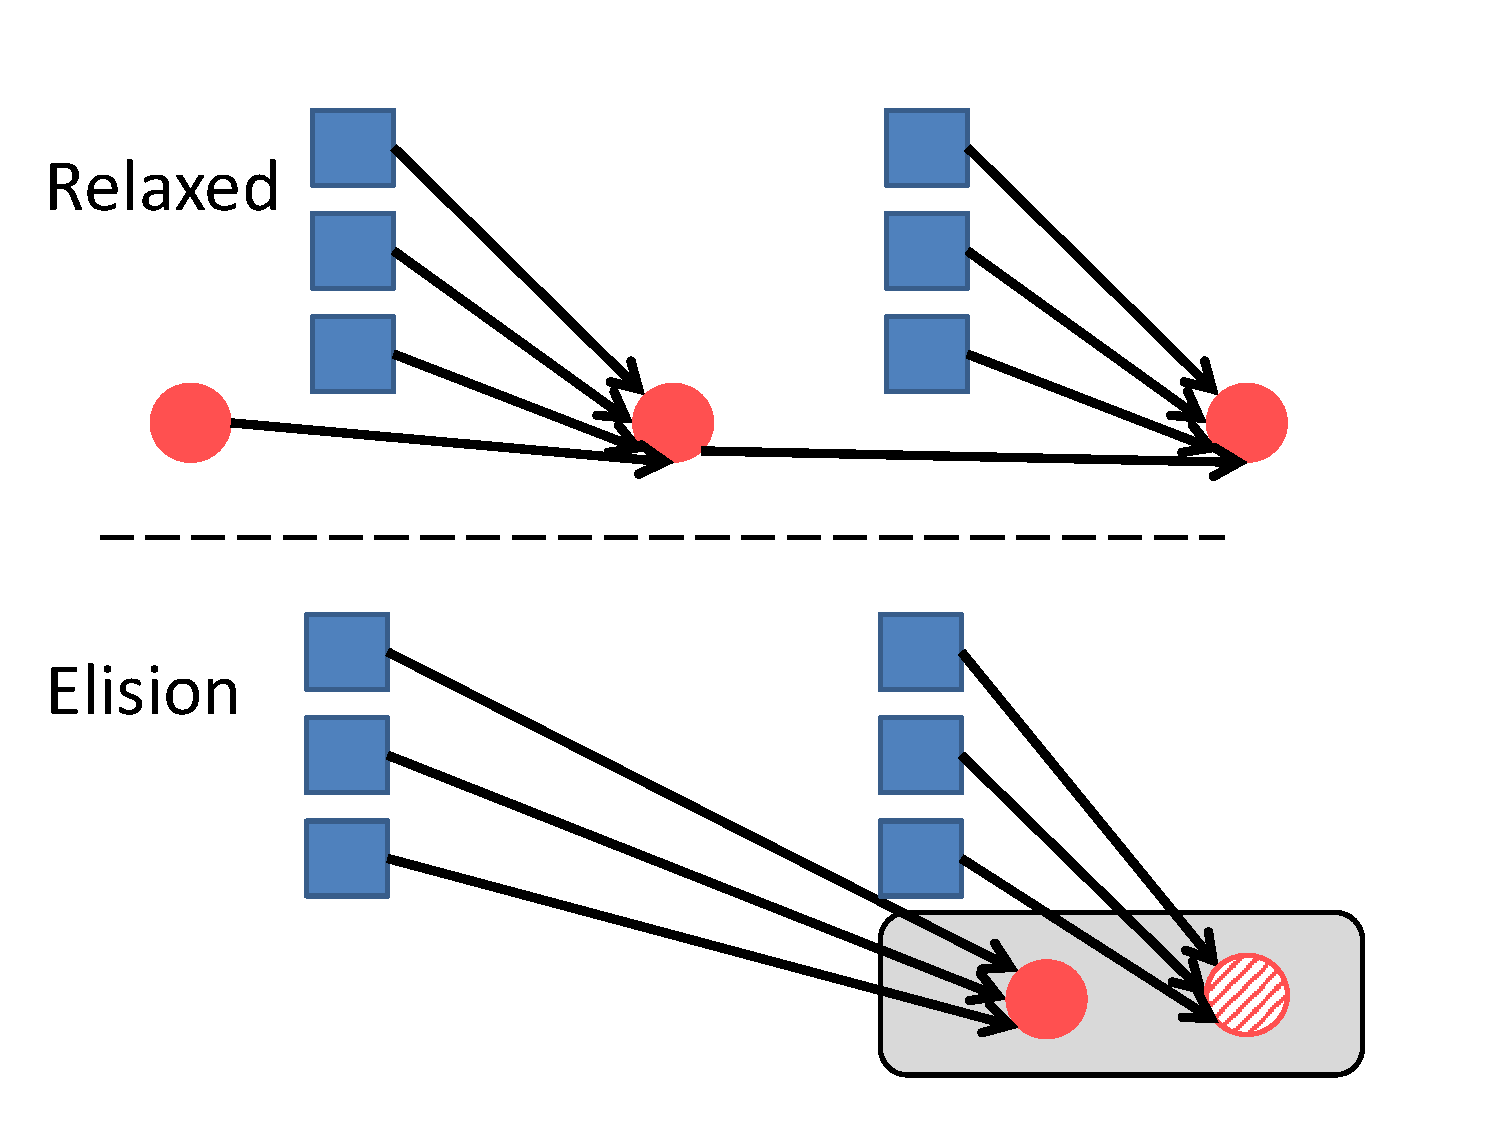
\includegraphics[width=\textwidth]{PMC_patterns/buffer_relaxed_elision.pdf}
\caption{Buffer execution under relaxed persistent consistency.  Relaxing persistent consistency by using LPO's cross-thread dependency tracking and TEO's single thread dependencies (top) allows buffer data to persist in parallel and forms a critical path chain only through counter persists.  Single threaded relaxed persistent consistency additionally requires precise barriers to describe non-sequential persist dependencies.  High performance systems may skip persists to the counter so long as all buffer persist dependencies are satisfied to the final counter value and all skipped values, effectively eliding persist epochs (bottom).}
\label{figure::buffer_relaxed_elision}
\end{figure}
